\section{Laser}\label{sec:laser}

A técnica de reconstrução baseada em laser é conhecida desde o século passado, pois oferecem uma alta qualidade geométrica de dados, os resultados são em tempo real e requer pouco tempo de captura de dados. 

Existem alguns tipos de reconstruções empregando lasers, baseados em volume (ressonância, tomografia, por exemplo \ref{fig:laservolume} ou em superfície (estereoscopia, {\it time of flight}, luz estruturada) . Neste caso, abordaremos o projeto de escaneamento da escultura de Michelangelo, David, que utiliza escaners baseados em superfícies, mais especificamente, utilizando luz estruturada.

\begin{figure}[!h]
	\centering
	%   \includegraphics[width=1.0\linewidth]{figs/3d-curve-sketch/system-diagram.eps}
	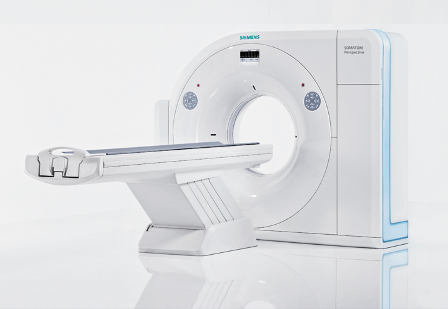
\includegraphics[width=1\linewidth]{figs/tomografia.png}
	\caption{%
	Exemplo de reconstrução à laser utilizando o método baseado em volume.
	%\cite{Cui:Theobalt:etal:PAMI2013,Pajdla:etal:ICCV2011}.
	}\label{fig:laservolume}
\end{figure}

Este projeto tem como motivação avançar a tecnologia de digitalização 3D e criar um acervo digital sobre alguns dos principais artefatos culturais. Foi utilizada uma tecnologia chamada de {\it rangefinder}, com uma equipe de mais de 30 professores, funcionários e estudantes da Universidade de Stanford desenvolveram algoritmos para combinar imagens de múltiplas gamas e cores, passaram os anos de 1998 e 1999 na Itália escaneando esclturas de Michelangelo. 

Pipeline:

O principal componente de {\it hardware} do sistema é um escaner de triangulação à laser, que é composto por 4 eixos motorizados, utiliza um laser, uma câmera de alcance, uma câmera de cores e uma luz branca, isso tudo acrescido de estruturas para estátuas grandes. O objetivo de um escaner deste porte era capturar marcas menores que um milímetro, das ferramentas utilizadas por Michelangelo em suas esculturas. 
Para isso foram testadas diversas resoluções, na qual foi decidido um espaçamento Y (ao longo da faixa do laser) de 1/4 mm e uma resolução Z (profundidade) de pelo menos duas vezes este valor. O que resultou em uma visualização de 14 cm de largura (ao longo da faixa do laser) por 14 cm de profundidade. Caso esta resolução fosse menor, as marcas de cinzelão ficariam borradas e se fosse maior, o conjunto de dados produzido seria gigantesco.
Felizmente, a maioria das estátuas feitas por Michelangelo foram esculpidas com um mármore encontrado em Carrara Statuario, uma pedra altamente uniforme, não direcional e constituída de grãos finos. Além disso, com exceção da "Noite", as esculturas não são polidas e cobertas por terra, o que aumenta a dispersão superficial e reduz a abaixo da superfície.
Neste contexto, a dispersão abaixo da superfície causa alguns problemas: não se pode assumir que a superfície é Lambertiana ideal (%CITAR LAMBERTIANO AQUI%
), mudou a forma com que a renderização dos modelos seriam feitos e diminuiu a qualidade de disposição de dados 


% Depois de testar várias resoluções, decidimos um espaçamento de amostra Y (ao longo da faixa laser) de 1/4 mm e uma resolução Z (profundidade) pelo menos duas vezes esta multa 1. Isso nos deu uma visão de 14 cm de largura (ao longo da faixa a laser ) por 14 cm de profundidade. Em retrospectiva, ficamos satisfeitos com a resolução que escolhemos; Qualquer coisa menor teria significativamente borrado as marcas de cinzelão de Michelangelo, e qualquer coisa maior teria tornado os nossos conjuntos de dados não gerenciáveis.

%FIGURA DAS FERRAMENTAS AQUI%


% The main hardware component of our system was a laser triangulation
% scanner and motorized gantry customized for digitizing
% large statues. Our requirements for this scanner were demanding;
% we wanted to capture chisel marks smaller than a millimeter, we
% wanted to capture them from a safe distance, and we wanted to
% reach the top of Michelangelo’s David, which is 23 feet tall on its
% pedestal. In the sections that follow, we describe the range and
% color acquisition systems of this scanner, its supporting mechanical
% gantry, and our procedure for calibrating it.

% O principal componente de hardware do nosso sistema foi um scanner de triangulação a laser e um pórtico motorizado personalizado para digitalizar grandes estátuas. Nossos requisitos para este scanner eram exigentes; queríamos capturar marcas de cinzelão menores do que um milímetro, queríamos capturá-las a uma distância segura, e queríamos chegar ao topo do David de Michelangelo, que tem 23 pés de altura no pedestal. Nas seções que se seguem, descrevemos os sistemas de aquisição de alcance e cor deste scanner, seu pórtico mecânico de suporte e nosso procedimento para calibrá-lo.

Primeiramente faz-se o escaneamento da geometria da escultura:
\begin{itemize}
\item{Alinhamento manual}
\item{ICP -- {\it Iterative Closest Point} para uma câmera existente} %CITAR ICP AQUI%
\item{ICP automático para todos os pares sobrepostos}
\item{Relaxação global para espalhar o erro}
\item{Reunir utilizando métodos volumétricos}
\end{itemize}


Após isso, ocorre o escaneamento e processamento das cores da escultura:

\begin{itemize}
\item{Compensação da iluminação do ambiente}
\item{Descarte de pixels com sombra ou especulares}
\item{Mapeia-se os vértices (uma cor por vértice)}
\item{Correção da irradiância e reflectância difusa}
\end{itemize}

Limitações:
\begin{ìtemize}
\item{Inter-reflexões são ignoradas}
\item{Dispersões subterrâneas são ignoradas}
\item{Tratamento difuso com Lambertiano} %CITAR TREATED DIFFUSED AS LAMBERTIAN%
\item{Usa superfícies normais agregadas}

\end{itemize}

O projeto não teve mais nenhum avanço desde o verão de 2004, por falta de financiamento. Como resultado, modelos de alta qualidade só existem do David na resolução de 1,0 mm (56 milhões de triângulos) e São Mateus a 0,25 mm (372 milhões de triângulos). Um modelo também existe para o Atlas em 0,25 mm (aproximadamente 500 milhões de triângulos), mas contém erros de alinhamento. Após 6 anos de trabalho estudantil remunerado e voluntário, existem modelos para cada um dos 1.186 fragmentos. Esses modelos, que totalizam quase 8 bilhões de polígonos, se encontram no próprio site da Universidade de Stanford %CITAR AQUI$. 

Também foram disponibilizadas algumas métricas sobre este projeto \ref{tab:metricasDavid}.

\begin{table}
\caption{Algumas métricas do projeto}
\label{tab:metricasDavid}
\begin{tabular}{|l|l|}
\hline
Números de objetos escaneados          & 10 estátuas + 2 edificações + 1,163 fragmentos de mapa  \\ \hline
Menor e maior objetos escaneados       & 1 polegada (fragmentos de mapa) e 23 pés (David)         \\ \hline
Resolução espacial dos dados                & 0.29mm para geometria, 0.125mm para cor              \\ \hline
Complexidade do maior conjunto de dados             & 2 bilhões de polígonos + 7,000 imagens (David)\\ \hline
Tamanho do maior conjunto de dados                    & 32 {\it gigabytes} (David)                  \\ \hline
Quantia total de dados capturados              & 250 {\it gigabytes}                                 \\ \hline
Tamanho do maior escaner                    & 24 pés de altura, 1800 libras de peso                  \\ \hline
Peso total do equipamento levado para a Itália & 4 toneladas                                              \\ \hline
Número de pessoas envolvidas                  & 32 (sem incluir subcontratantes e colaboradores) \\ \hline
Tempo médio para escaneamento              & 1 semana (exceto o David, que levou 1 mês)       \\ \hline
Tempo total de escaneamento                 & 5,000 horas de trabalho                                   \\ \hline
Total de tempo para processamento de dados          & 4,000 horas de trabalho (até agora)                            \\ \hline
Custo do projeto                          & \$2,000,000                                         \\ \hline
\end{tabular}
\end{table}
%COLOCAR FOTOS DAVID%
Porém, devido ao seu alto custo com equipamentos, com {\it softwares} e sem falar na necessidade de estações robustas para armazenamento dos dados e para esacaneamento de patrimônios, outras técnicas foram emergindo com o passar dos anos, como a fotogrametria, que será abordada mais tarde neste documento.